\documentclass[12pt]{article}
\usepackage[vmargin=20mm, hmargin=15mm]{geometry} 
\usepackage{multicol}
\usepackage{datetime}
\usepackage{array}
\usepackage{lipsum}
\usepackage{graphicx}
\usepackage{mwe}
%\usepackage{url}
%\usepackage{hyperref}
%\usepackage[svgnames]{xcolor}
%\hypersetup{
 % colorlinks,
 % urlcolor=Blue}
  
\geometry{a4paper} 
\frenchspacing
\parindent 0pt
\parskip 6pt
\setlength\columnsep{15pt}

\newcommand{\docvec}{\texttt{doc2vec}}
\newcommand{\wordvec}{\texttt{word2vec}}

%%% BEGIN DOCUMENT
\begin{document}
\centerline{\large NLP Assignment 2 Report}
\vspace{0.1in}
\centerline{\Large\bf Doc2Vec for Sentiment Detection of Reviews}
\vspace{0.1in}
\centerline{\large {\bf{Z\'ebulon Goriely, Queens', zg258}}}
\vspace{0.1in}
\centerline{\large {\today}}
\vspace{0.05in}
\centerline{Word Count: 987\footnote{\emph{texcount docs/assignment2/report.tex}}}
\vspace{0.2in}

\makeatletter
\newenvironment{tablehere}
  {\def\@captype{table}}
  {}

\newenvironment{figurehere}
  {\def\@captype{figure}}
  {}
\makeatother

%%% BEGIN BODY OF TEXT
\begin{multicols}{2}

\section{Introduction}

In a 2014 paper, based on \wordvec, Le and Mikolov \cite{le2014distributed} introduced \docvec~for learning embeddings for sequences of words. Here, we investigate the use of \docvec~document vectors in the task of sentiment detection, using a Support Vector Machine (SVM) classifier.

We compare the success of the classifier trained with \docvec~vectors to the same classifier trained\footnote{We were given a dataset of movie reviews in the framework of a course in NLP} with simple word-frequency and one-hot coded vectors. Finally, we examine means of qualitatively analysing the behaviour of \docvec, in particular how sentiment-coding adjectives are represented.

\section{Background}

To classify reviews, we use an SVM classifier trained and tested on document vectors.

Previously, we looked at document vectors where each document $d$ was represented as a vector $\vec{d} := (n_{1}(d), n_{2}(d),\ldots,n_{m}(d))$ where $n_{i}(d)$ is the occurrences $f_{i}$ of document $d$.

Selecting unigrams as our feature, we will compare the performance of training and testing an SVM classifier on:
\vspace{-\topsep}
\begin{itemize}
\setlength{\parskip}{0pt}
\setlength{\itemsep}{0pt plus 1pt}
	\item frequency-based bag-of-words document vectors
	\item one-hot encoded bag-of-words document vectors
	\item vectors inferred from a trained \docvec~model
\end{itemize}
\vspace{-\topsep}

\subsection{Doc2Vec}

Mikolov et al. introduced the ideas of skipgrams and \wordvec~to create compact vector-space representations of words \cite{mikolov2013distributed}. Unlike our frequency-based document vectors and one-hot encoded vectors, the dimensions of the vectors are not directly interpretable.

Le and Mikolov extended this idea to \docvec~which learns embeddings of \emph{sequences} of words. A key feature is that it is agnostic to granularity, generating fixed-length vectors from variable-length pieces of text. In this case, we train \docvec~to output document embeddings, a new type of vector that Le and Mikolov claim is effective for sentiment analysis.

The two architectures in \docvec~are the distributed memory and distributed bag of words model which are closely correlated to the \wordvec~ and skip-gram models respectively.
\\\\
\begin{table*}[t]
\centering
 \begin{tabular}{ r l c}
 \bf{Hyperparameter} & \bf{Description} & \bf{Best Value} \\ [0.5ex] 
 \hline
Vector Size &  Dimension of word vectors & 124 \\ 
Window Size & Left/right context window size & 6 \\
Min Count & Minimum frequency threshold for word types & 20 \\
Negative Sample & No. of negative word samples & 0 \\
Epoch & Number of training epochs & 5 \\
\end{tabular}
\caption{A description of \texttt{doc2vec} hyperparameters and the best values found for this task.} \label{table:params}
\end{table*}

\begin{table*}[t]
\centering
 \begin{tabular}{|c|c|c|c|} 
 \hline
  & Unigram-frequency & One-hot unigrams & doc2vec \\ [0.5ex] 
 \hline\hline
Unigram-frequency & 1 &  $2.00\times 10^{-4}$ & $2.00\times 10^{-4}$\\
 \hline
One-hot unigrams & $2.00\times 10^{-4}$ & 1  & $1.60\times 10^{-3}$\\
 \hline
doc2vec & $2.00\times 10^{-4}$ & $1.60\times 10^{-3}$ & 1 \\
 \hline
\end{tabular}
\caption{The p-values from a Monte-Carlo permutation test with a significance level of $k = 0.01$.} \label{table:p-values}
\end{table*}

\vspace{-3mm}

\subsection{Support Vector Machine}

Pang et al.~\cite{pang2002thumbs} introduced the use of SVM classifiers for sentiment analysis.

Letting $c_{j} \in \{1, -1\}$ (corresponding to positive and negative) be the correct class of document $d_{j}$, the procedure finds the hyperplane represented by vector $\vec{w}$ which divides document vectors into  two classes.

Once trained, classification proceeds by determining which side of the hyperplane each $d_{i}$ falls on. We use Joachim's (1999) $SVM^{light}$ package\footnote{http://svmlight.joachims.org}, using default parameters.

\section{Method}

We implemented our SVM classifier using Python\footnote{https://github.com/ZGoriely/cambridge-nlp}. For the \docvec~implementation, we use the gensim library\footnote{https://radimrehurek.com/gensim}.

We train the \docvec~model on a large external corpora of 100,000 movie reviews provided by the Stanford Large Movie Review Dataset \cite{maas-EtAl:2011:ACL-HLT2011}. In a 2014 evaluation of \docvec~, Lau and Baldwin \cite{lau2016empirical} suggest relevant parameters to use for training, as described in Table \ref{table:params}. 

To tune our parameters we set aside a validation corpus comprising of 10\% of our 2000 movie review dataset. For each set of parameters chosen, we trained \docvec~on the 100,000 unlabelled files, used this model to generate vectors to train SVM on 90\% of our 2000 movie review dataset and tested on this validation corpus. The validation corpus was never used for training and once suitable parameters were found, it was not used for testing (testing was done through cross-validation on the remaining 1800 reviews).

Parameters were initially chosen using Lau and Baldwin's suggestions. We then tested a range of values for each parameter, in order to increase the accuracy when testing on the validation corpus. 

During this process we also found that the distributed bag of words (\texttt{dbow}) model was more effective than the distributed memory (\texttt{dm}) model and that using hierarchical softmax also improved performance. The best parameters found from this process are shown in Table \ref{table:params}, giving an accuracy of 89\% on the validation corpus.

\section{Results}

%%% DATA
\begin{tablehere}
\centering
 \begin{tabular}{| c | c | c|} 
 \hline
   & Vector Type & Accuracy \\ [0.5ex] 
 \hline\hline
 (1) & Unigram-frequency & 75.9\\ 
 \hline
 (2) & One-hot unigrams & 86.7 \\
 \hline
 (3) & doc2vec & 89.3 \\
 \hline
\end{tabular}
\caption{Average ten-fold cross-validation accuracies, in percent. Dataset: 1800 movie reviews.} \label{table:accuracies}
\end{tablehere}

We ran ten-fold cross-validation for our three experiments as detailed in Table \ref{table:accuracies}, using our 1800 movie reviews.

The result of 89.3\% achieved using \docvec~ is significantly better than the 75.9 and 86.7 achieved by the frequency vectors and one-hot vectors respectively. The significance was calculated using a permutation test, with p-values recorded in Table \ref{table:p-values}.

\begin{figure*}[t]
    \centering
    \begin{minipage}{0.49\textwidth}
       \centering
       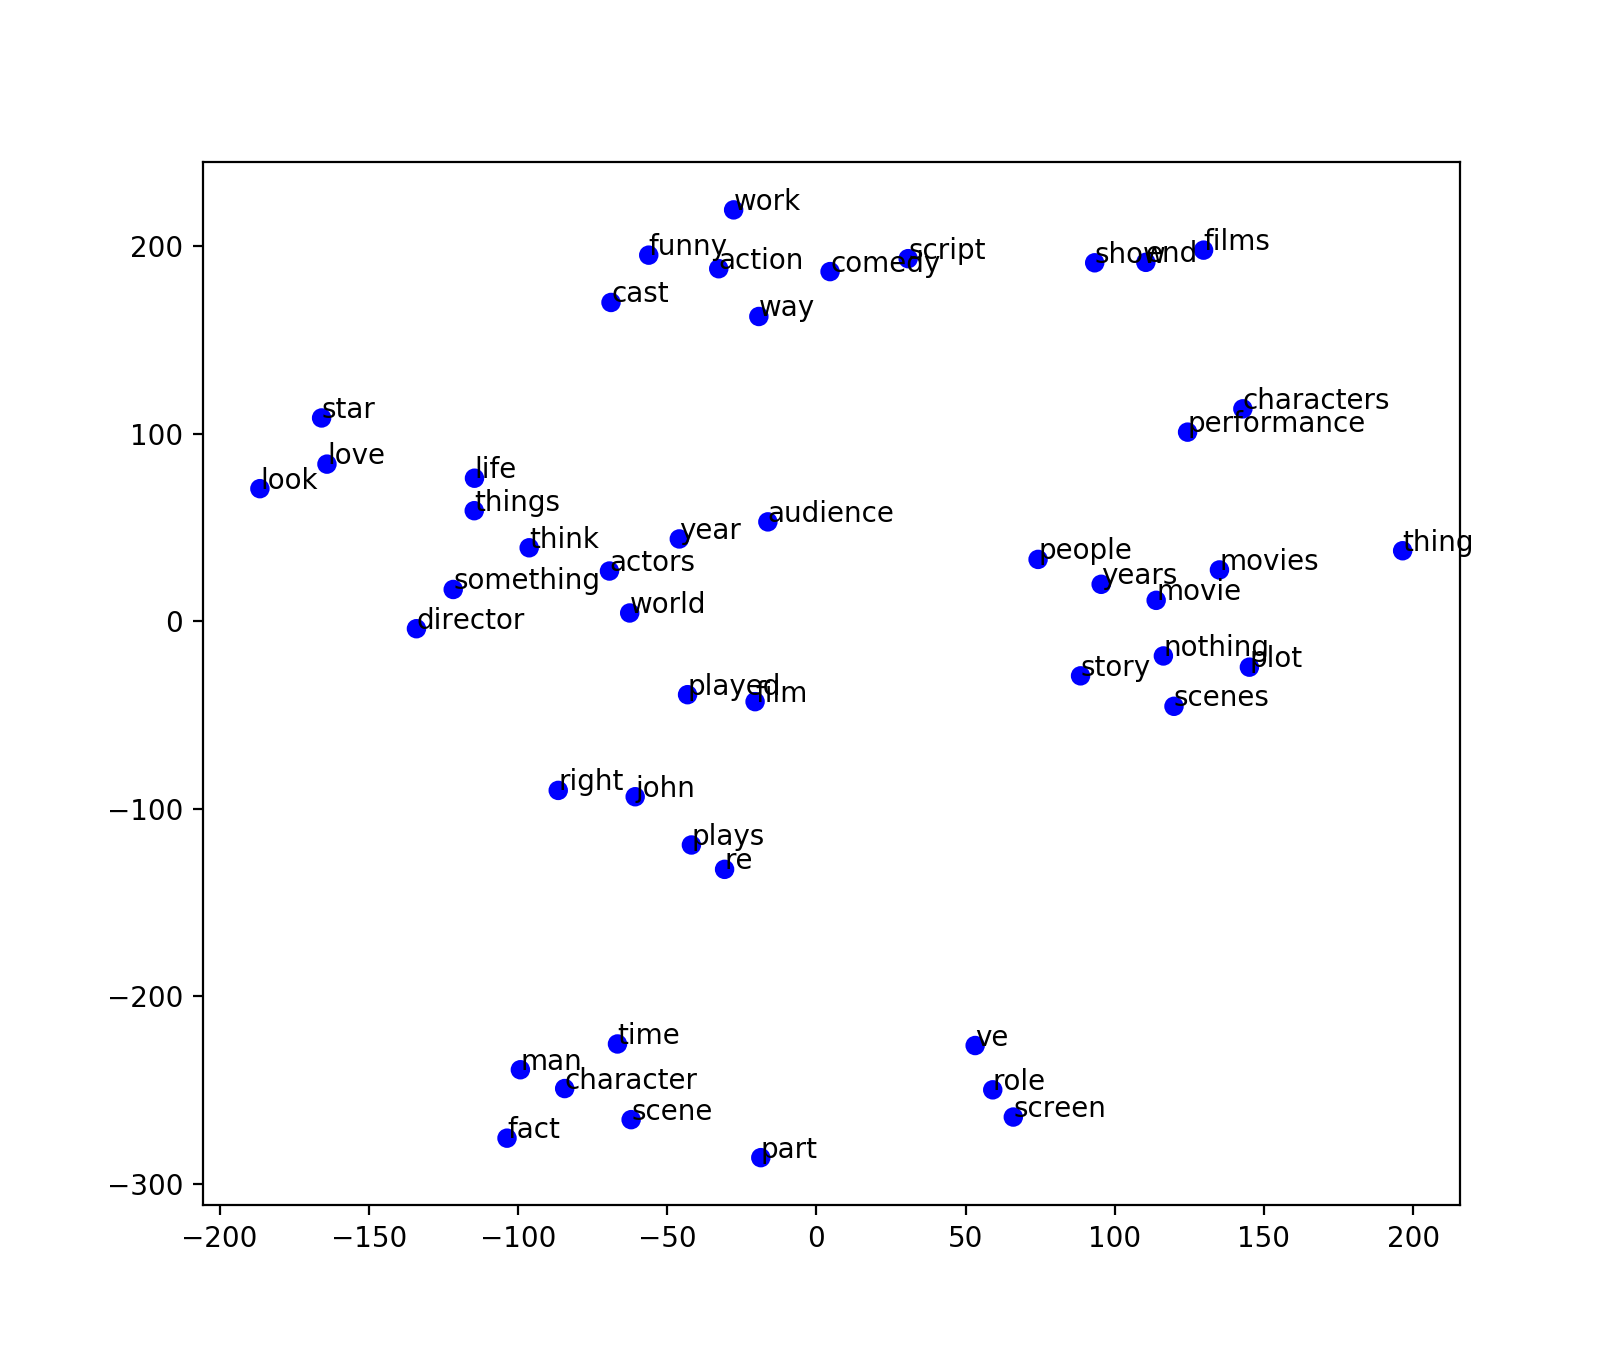
\includegraphics[width=1\textwidth]{figs/nouns.png}
       \caption{Two-dimensional t-SNE projection of doc2vec embeddings of the 50 most frequent nouns}
       \label{figure:nouns}
    \end{minipage}\hfill
    \begin{minipage}{0.49\textwidth}
       \centering
       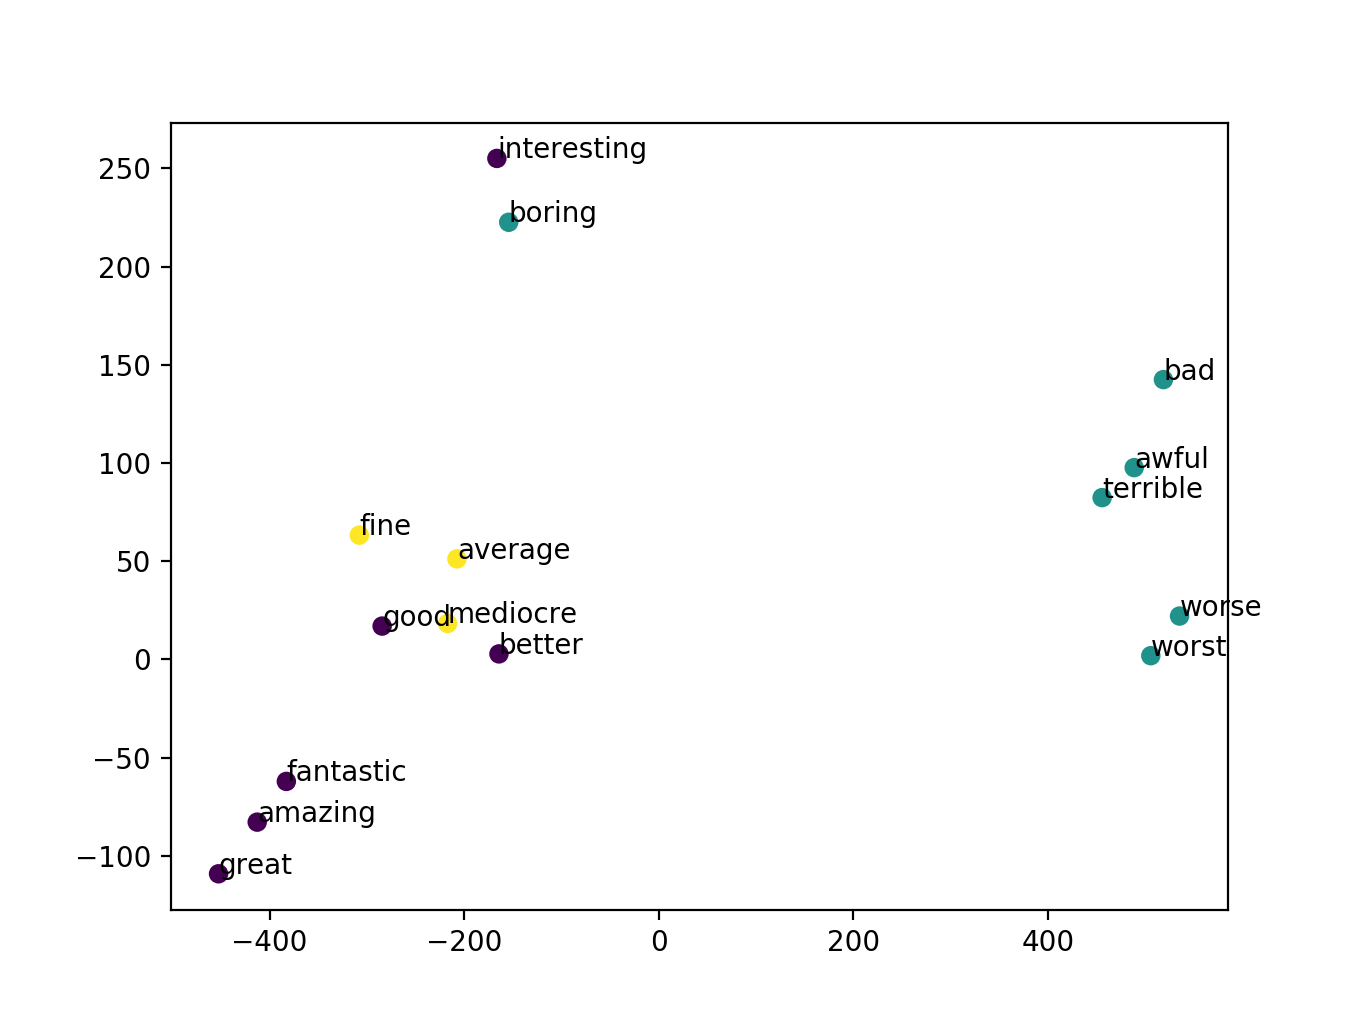
\includegraphics[width=1\textwidth]{figs/sentiment.png}
       \caption{Two-dimensional t-SNE projection of doc2vec adjective embeddings}
       \label{figure:sentiments}
    \end{minipage}
\end{figure*}

\section{Discussion}

Our results show that the more complicated \docvec~model, taking the \emph{context} of words into account, performs better at sentiment analysis than the simple naive bag-of-word models for generating document vectors. Using T-sne and heatmap graphs, we can qualitatively examine what the model is doing.

By plotting the 50 most frequent nouns in our 2000 files using t-SNE in Figure \ref{figure:nouns}, we see how \docvec~learns context. Nouns used in the same context such as \emph{plot, story} and \emph{man, character} are grouped together and are thus represented by similar vectors in the \docvec~embedded vector space.

We hypothesise that \docvec~learns sentiments of common adjectives from their usage in the positive and negative files that \docvec~is trained on. We plot these adjectives using t-SNE in Figure \ref{figure:sentiments}.

\begin{tablehere}
\centering
 \begin{tabular}{| c | c | c|}  
 \hline
Word & Positive & Negative \\ [0.5ex] 
 \hline\hline
 amazing & 2004 & 516 \\
 \hline
 good & 15025 & 14728 \\ 
 \hline
bad & 3747 & 14726 \\
 \hline
average & 595 & 831 \\
 \hline
\end{tabular}
\caption{Occurrences of words in positive and negative training files} \label{table:occurrences}
\end{tablehere}

We observe that the model seems to learn the sentiment of these adjectives. \emph{Fantastic, amazing, great} are grouped together and \emph{bad, awful, terrible, worse, worst} are also grouped. Interestingly, the neutral adjectives \emph{fine, average, mediocre} seem to be grouped with the positive adjectives \emph{good, better}. This may be due to the comparative occurrence of these adjectives in positive and negative files. As seen in Table \ref{table:occurrences}, the words \emph{amazing} and \emph{bad} dominate in positive and negative files respectively whereas the words \emph{good} and \emph{average} are distributed more evenly between positive and negative files.

Li et al. \cite{li2015visualizing} proposed a method to visualise indicator words by plotting the variance of word vectors in a sentence against each other. In Figure \ref{figure:goodbad}, we plot a variance visualisation of the sentence \emph{``this has to be one of the greatest movies of all time''}; each grid corresponds to $ ||e_{i,j} - \frac{1}{N_{s}} \sum_{i'\in N_{s}}e_{i',j} ||^{2} $ where $e_{i,j}$ denotes the value for $j$th dimension of word $i$ and $N$ denotes the number of token within the sentences. This gives us the word \emph{greatest} as the strongest indicator for this sentence.

A heat-map visualisation of three short reviews, shown in Figure \ref{figure:goodbad}, reveals another analysis that \docvec~learns sentiment; the neutral review seems to lie between the heat-maps of the positive and negative reviews.

\begin{figure*}[t]
    \centering
    \begin{minipage}{0.49\textwidth}
       \centering
       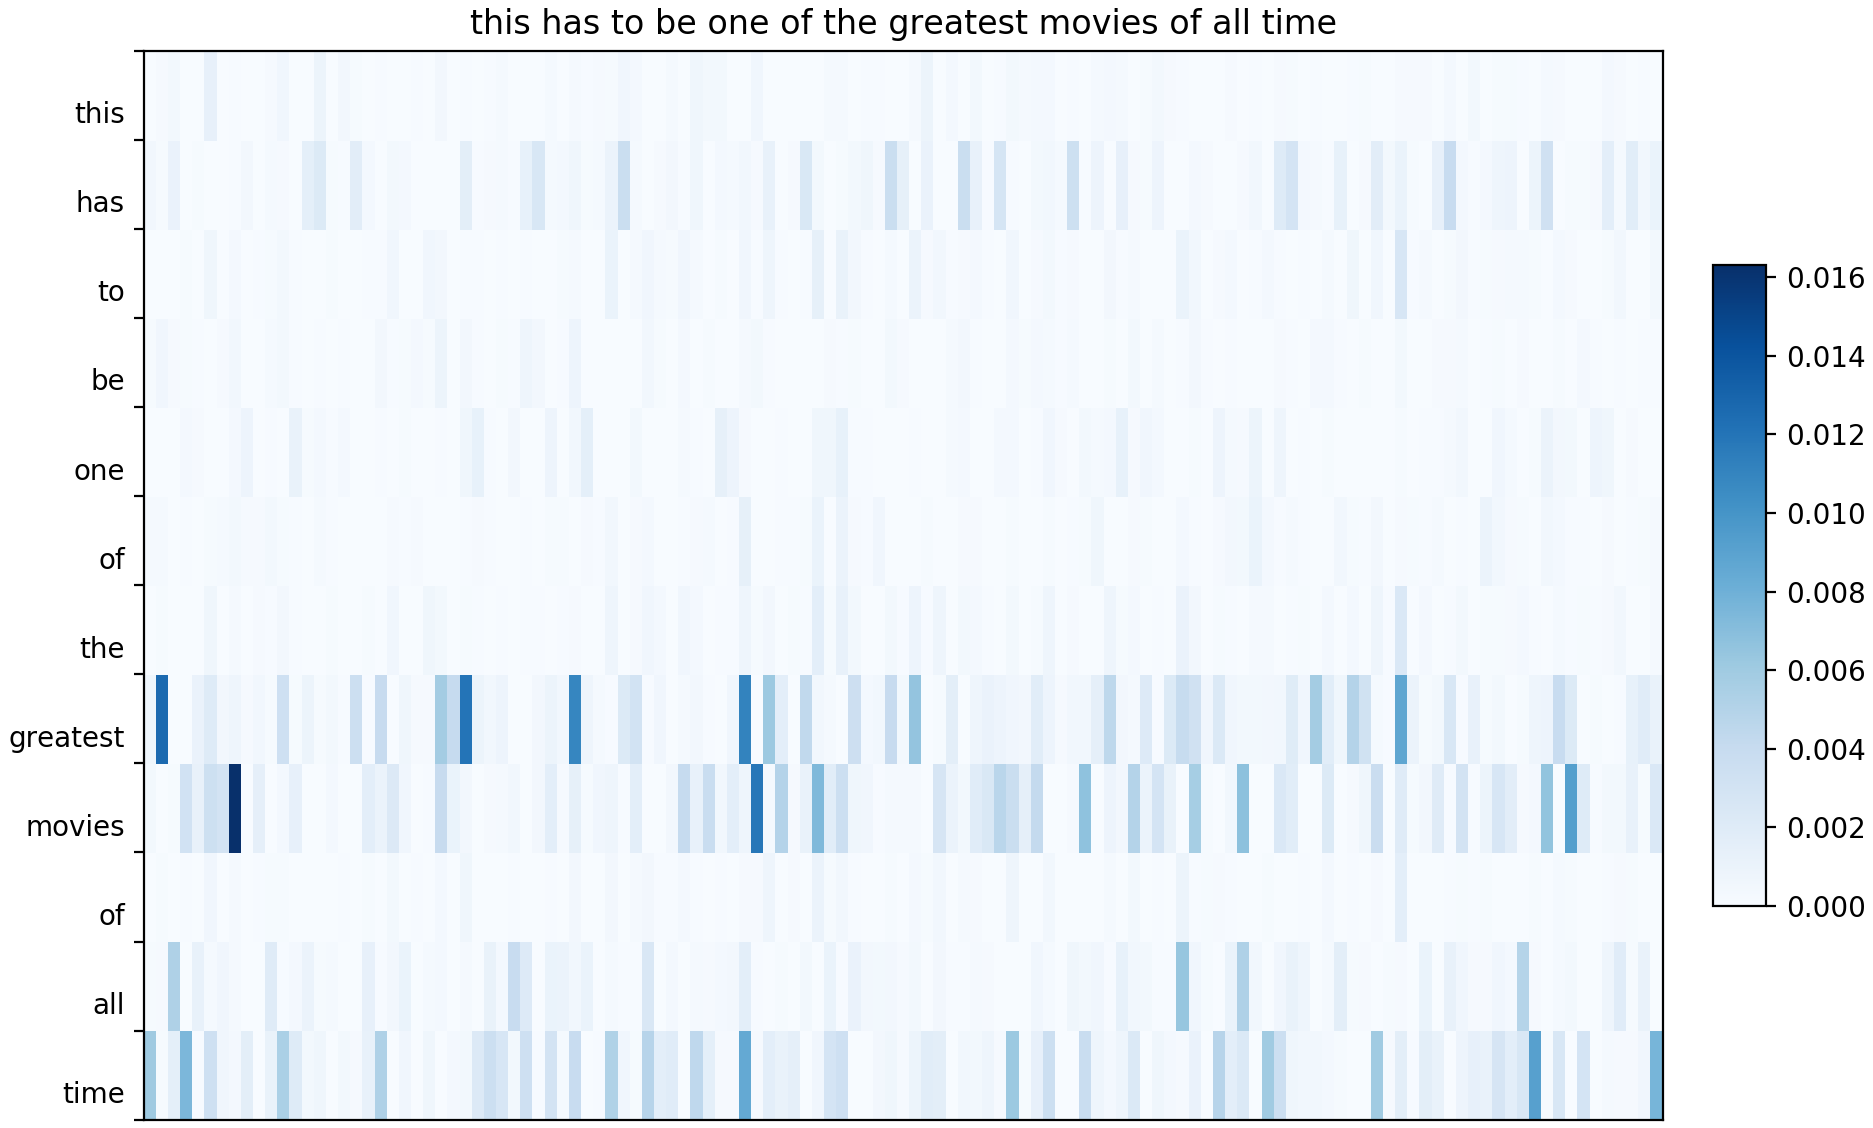
\includegraphics[width=1\textwidth]{figs/greatest.png}
       \caption{Variance visualisation of a single-sentence review}
       \label{figure:greatest}
    \end{minipage}\hfill
    \begin{minipage}{0.49\textwidth}
       \centering
       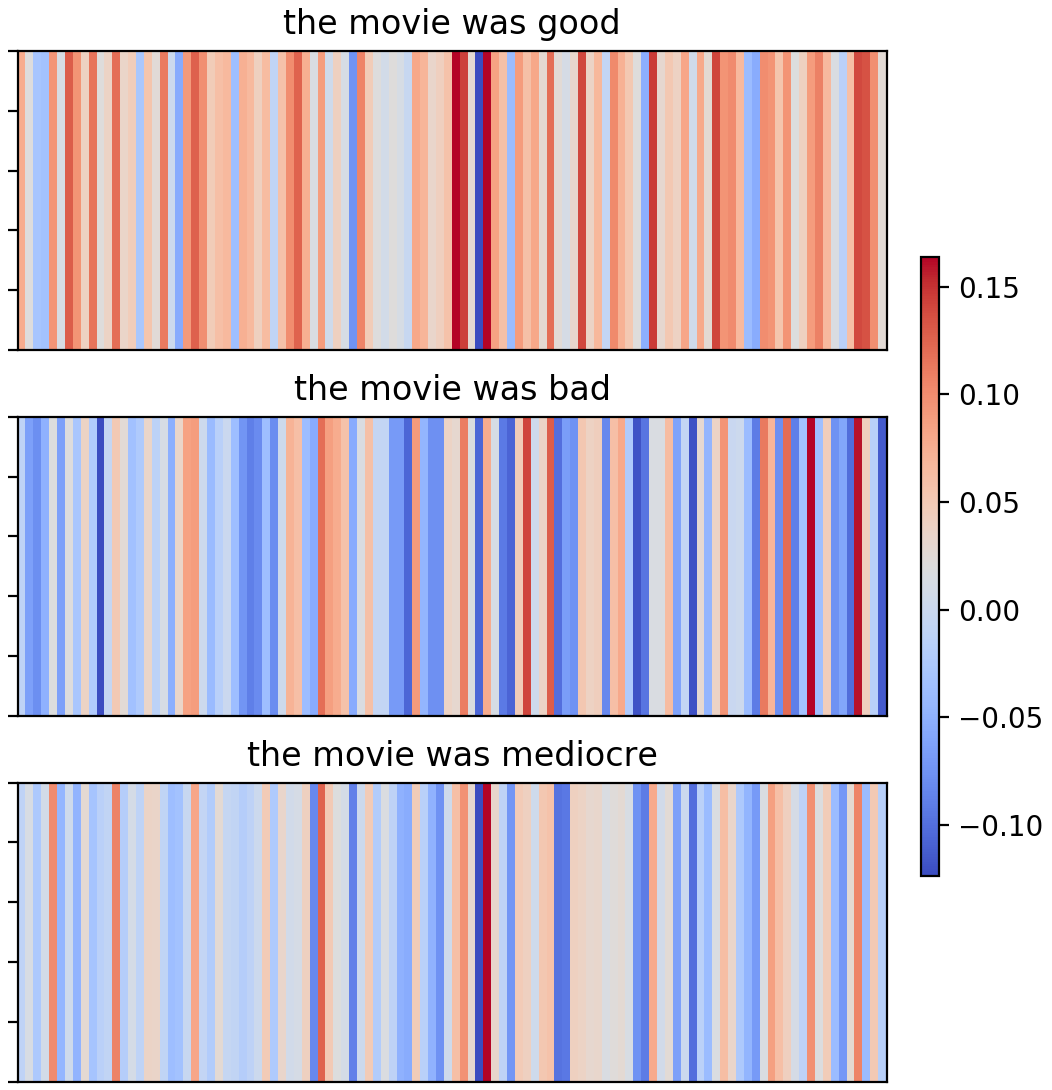
\includegraphics[width=1\textwidth]{figs/goodbad.png}
       \caption{Heat-map visualisation of a good, bad and neutral sentiments}
       \label{figure:goodbad}
    \end{minipage}
\end{figure*}

\section*{Conclusion}

We have shown how using \docvec~vectors in an SVM classifier outperforms naive frequency-based vectors and one-hot vectors. We further qualitatively analysed the behaviour of \docvec, finding that the model learns sentiment through occurence of adjectives in positive and negative documents.

\bibliography{refs}
\bibliographystyle{plain}

\end{multicols}
\end{document}